\documentclass[a4paper,twocolumn]{IEEEtran}

\usepackage{amsmath,amsfonts,amssymb}
\usepackage{graphicx,float,subfig}
\usepackage{booktabs}
\usepackage[colorlinks=true]{hyperref}

\author{Oliver Kirkpatrick\footnote{oliver.kirkpatrick@rmit.edu.au}}

\begin{document}
    \title{Analysis of Gamma Ray Spectra from Reference Isotopes with Multi-Channel Analyzers}
    \author{\IEEEauthorblockA{Oliver Kirkpatrick}
    \\
    \IEEEauthorblockA{School of Engineering, RMIT University\\
    Email: s3725341@student.rmit.edu.au}}

    \maketitle
    \begin{abstract}
        stuff
    \end{abstract}
    \section{Results and Discussion}
    \subsection{Calibration Process}
    \subsection{Background Radiation}
    \begin{figure}[H]
        \centering
        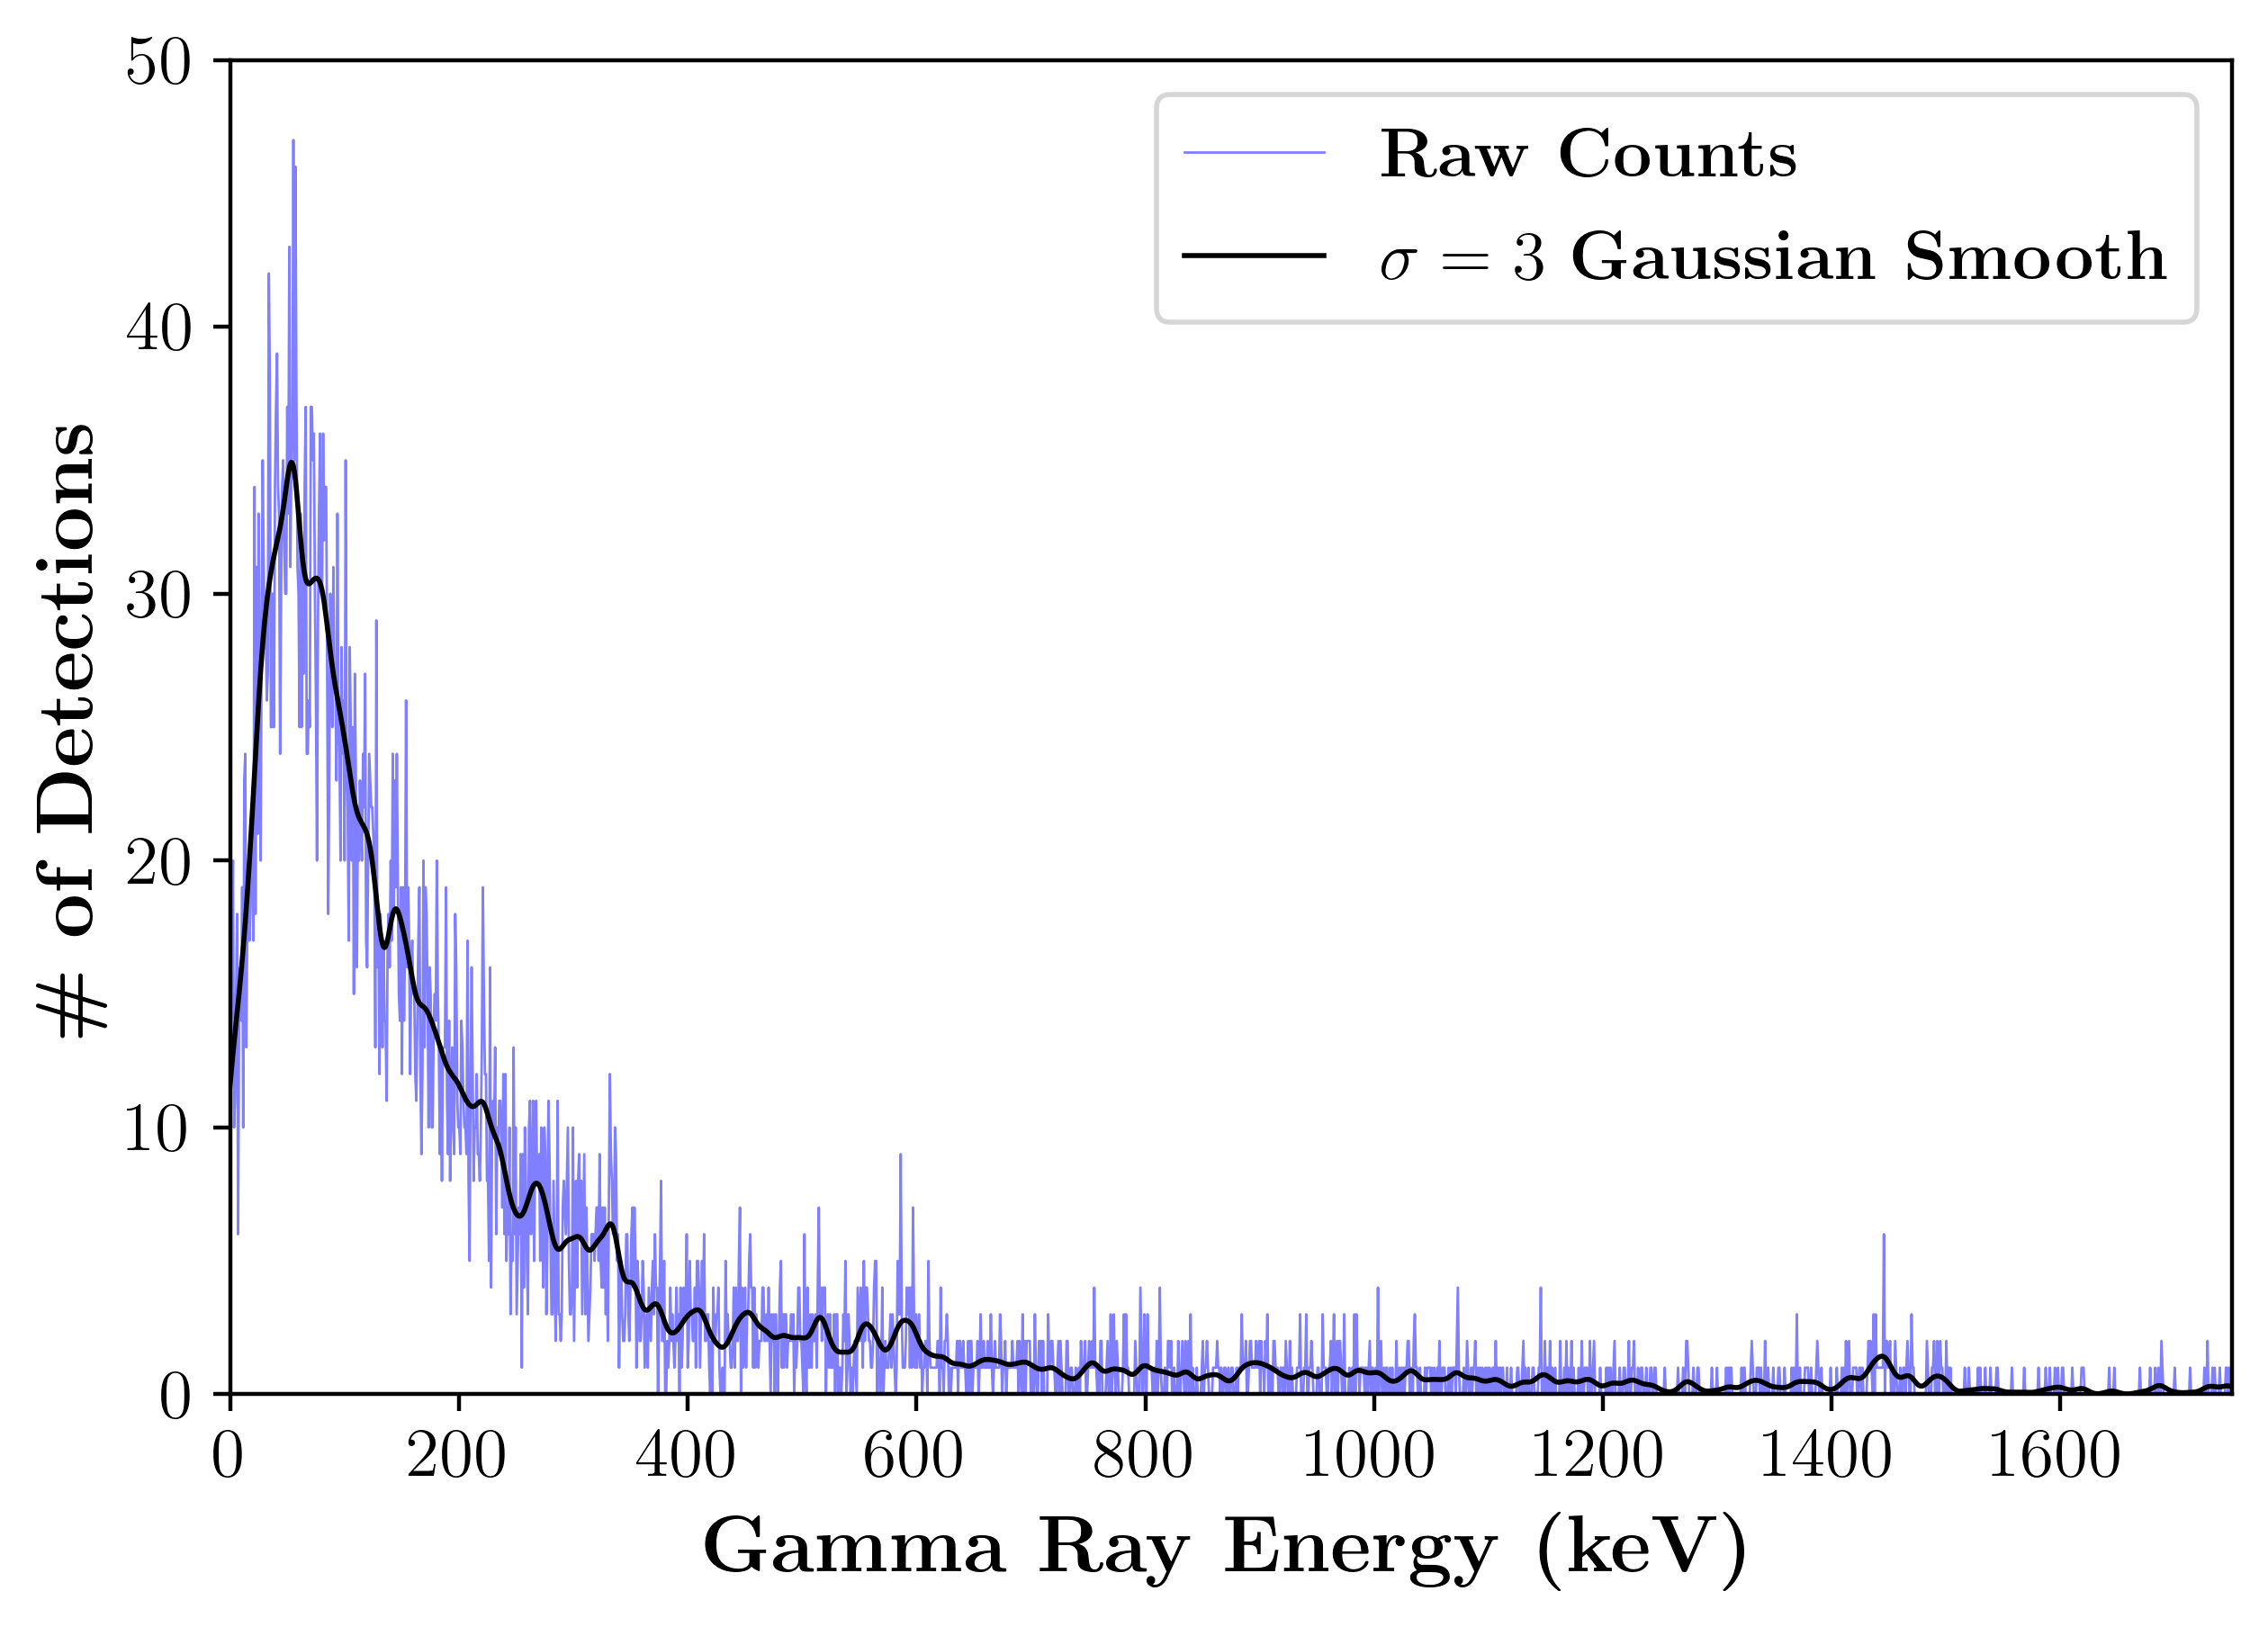
\includegraphics[width=0.95\linewidth]{figures/background_counts_overlay.png}
        \caption{Background radiation profile.}
    \end{figure}
    \subsection{Analysis of Unknown Sample}
    \begin{figure}[H]
        \centering
        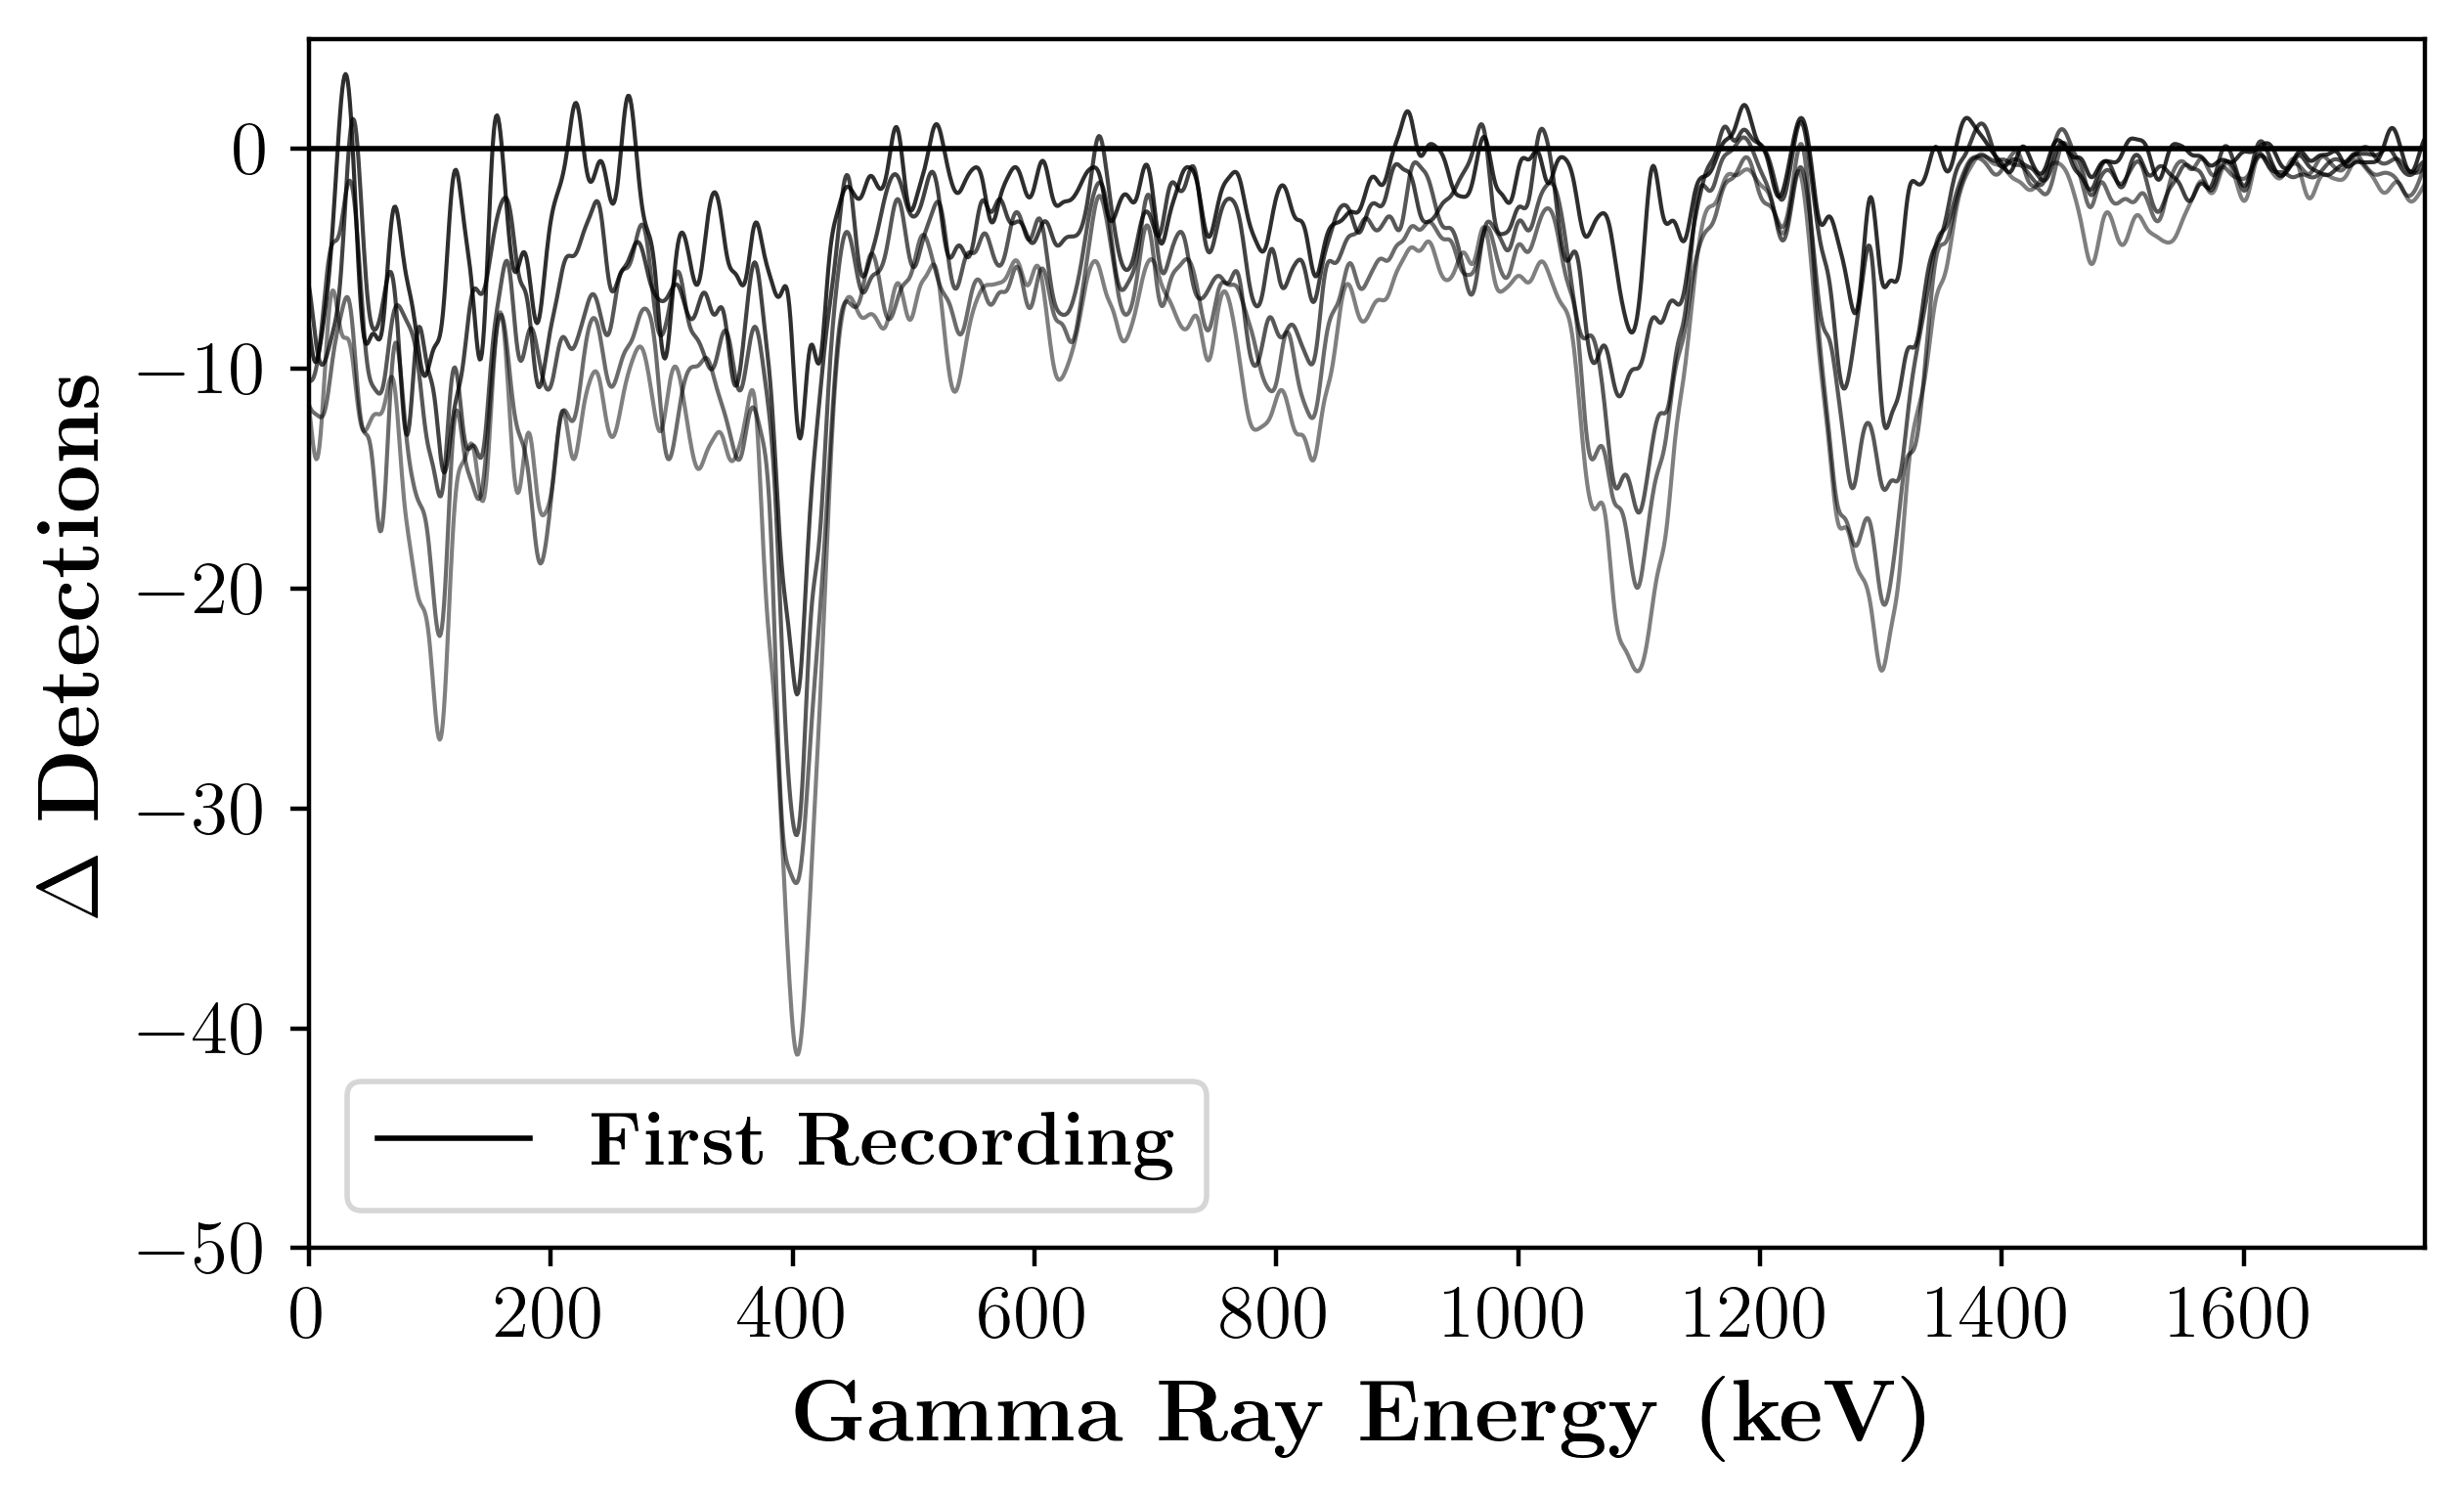
\includegraphics[width=0.95\linewidth]{figures/difference_counts_smooth.png}
    \end{figure}

    \begin{table*}[t]
        \centering
        \caption{Total counts and peak energies with with increasing time since first measurement.}
        \begin{tabular}{c c c c c c c}
            \toprule
            \textbf{Sample Number} & $T+$ \textbf{(s)} & \textbf{Total Counts} & \textbf{Peak 1 Energy} & \textbf{Peak 2 Energy} & \textbf{Peak 3 Energy} & \textbf{Peak 4 Energy} \\
            \midrule
            1 & 0s & 68493 & 401.24 keV &  815.92 keV & 1096.59 keV & 1296.46 keV \\
            2 & 420s & 63755 & 400.52 keV & 799.32 keV & 1106.59 keV & 1295.25 keV \\
            3 & 819s & 59850 & 401.25 keV & 796.80 keV & 1099.32 keV  & 1293.16 keV \\
            4 & 1199s & 56863 & 400.35 keV & 759.04 keV & 1097.07 keV & 1295.73 keV \\
            5 & 1559s & 53111 & 401.94 keV & 805.54 keV & 1104.55 keV & 1296.78 keV \\
            6 & 1936s & 50483 & 400.41 keV & 812.17 keV & 1085.92 keV & 1292.84 keV \\
            \bottomrule
        \end{tabular}
        \label{tab:counts_v_time}
    \end{table*}
    \onecolumn
    \appendix
    \begin{figure}[H]
        \centering
        \subfloat[Recording 1, hh:mm:ss, $T+$ minutes\label{subfig:mystery-recording-1}]{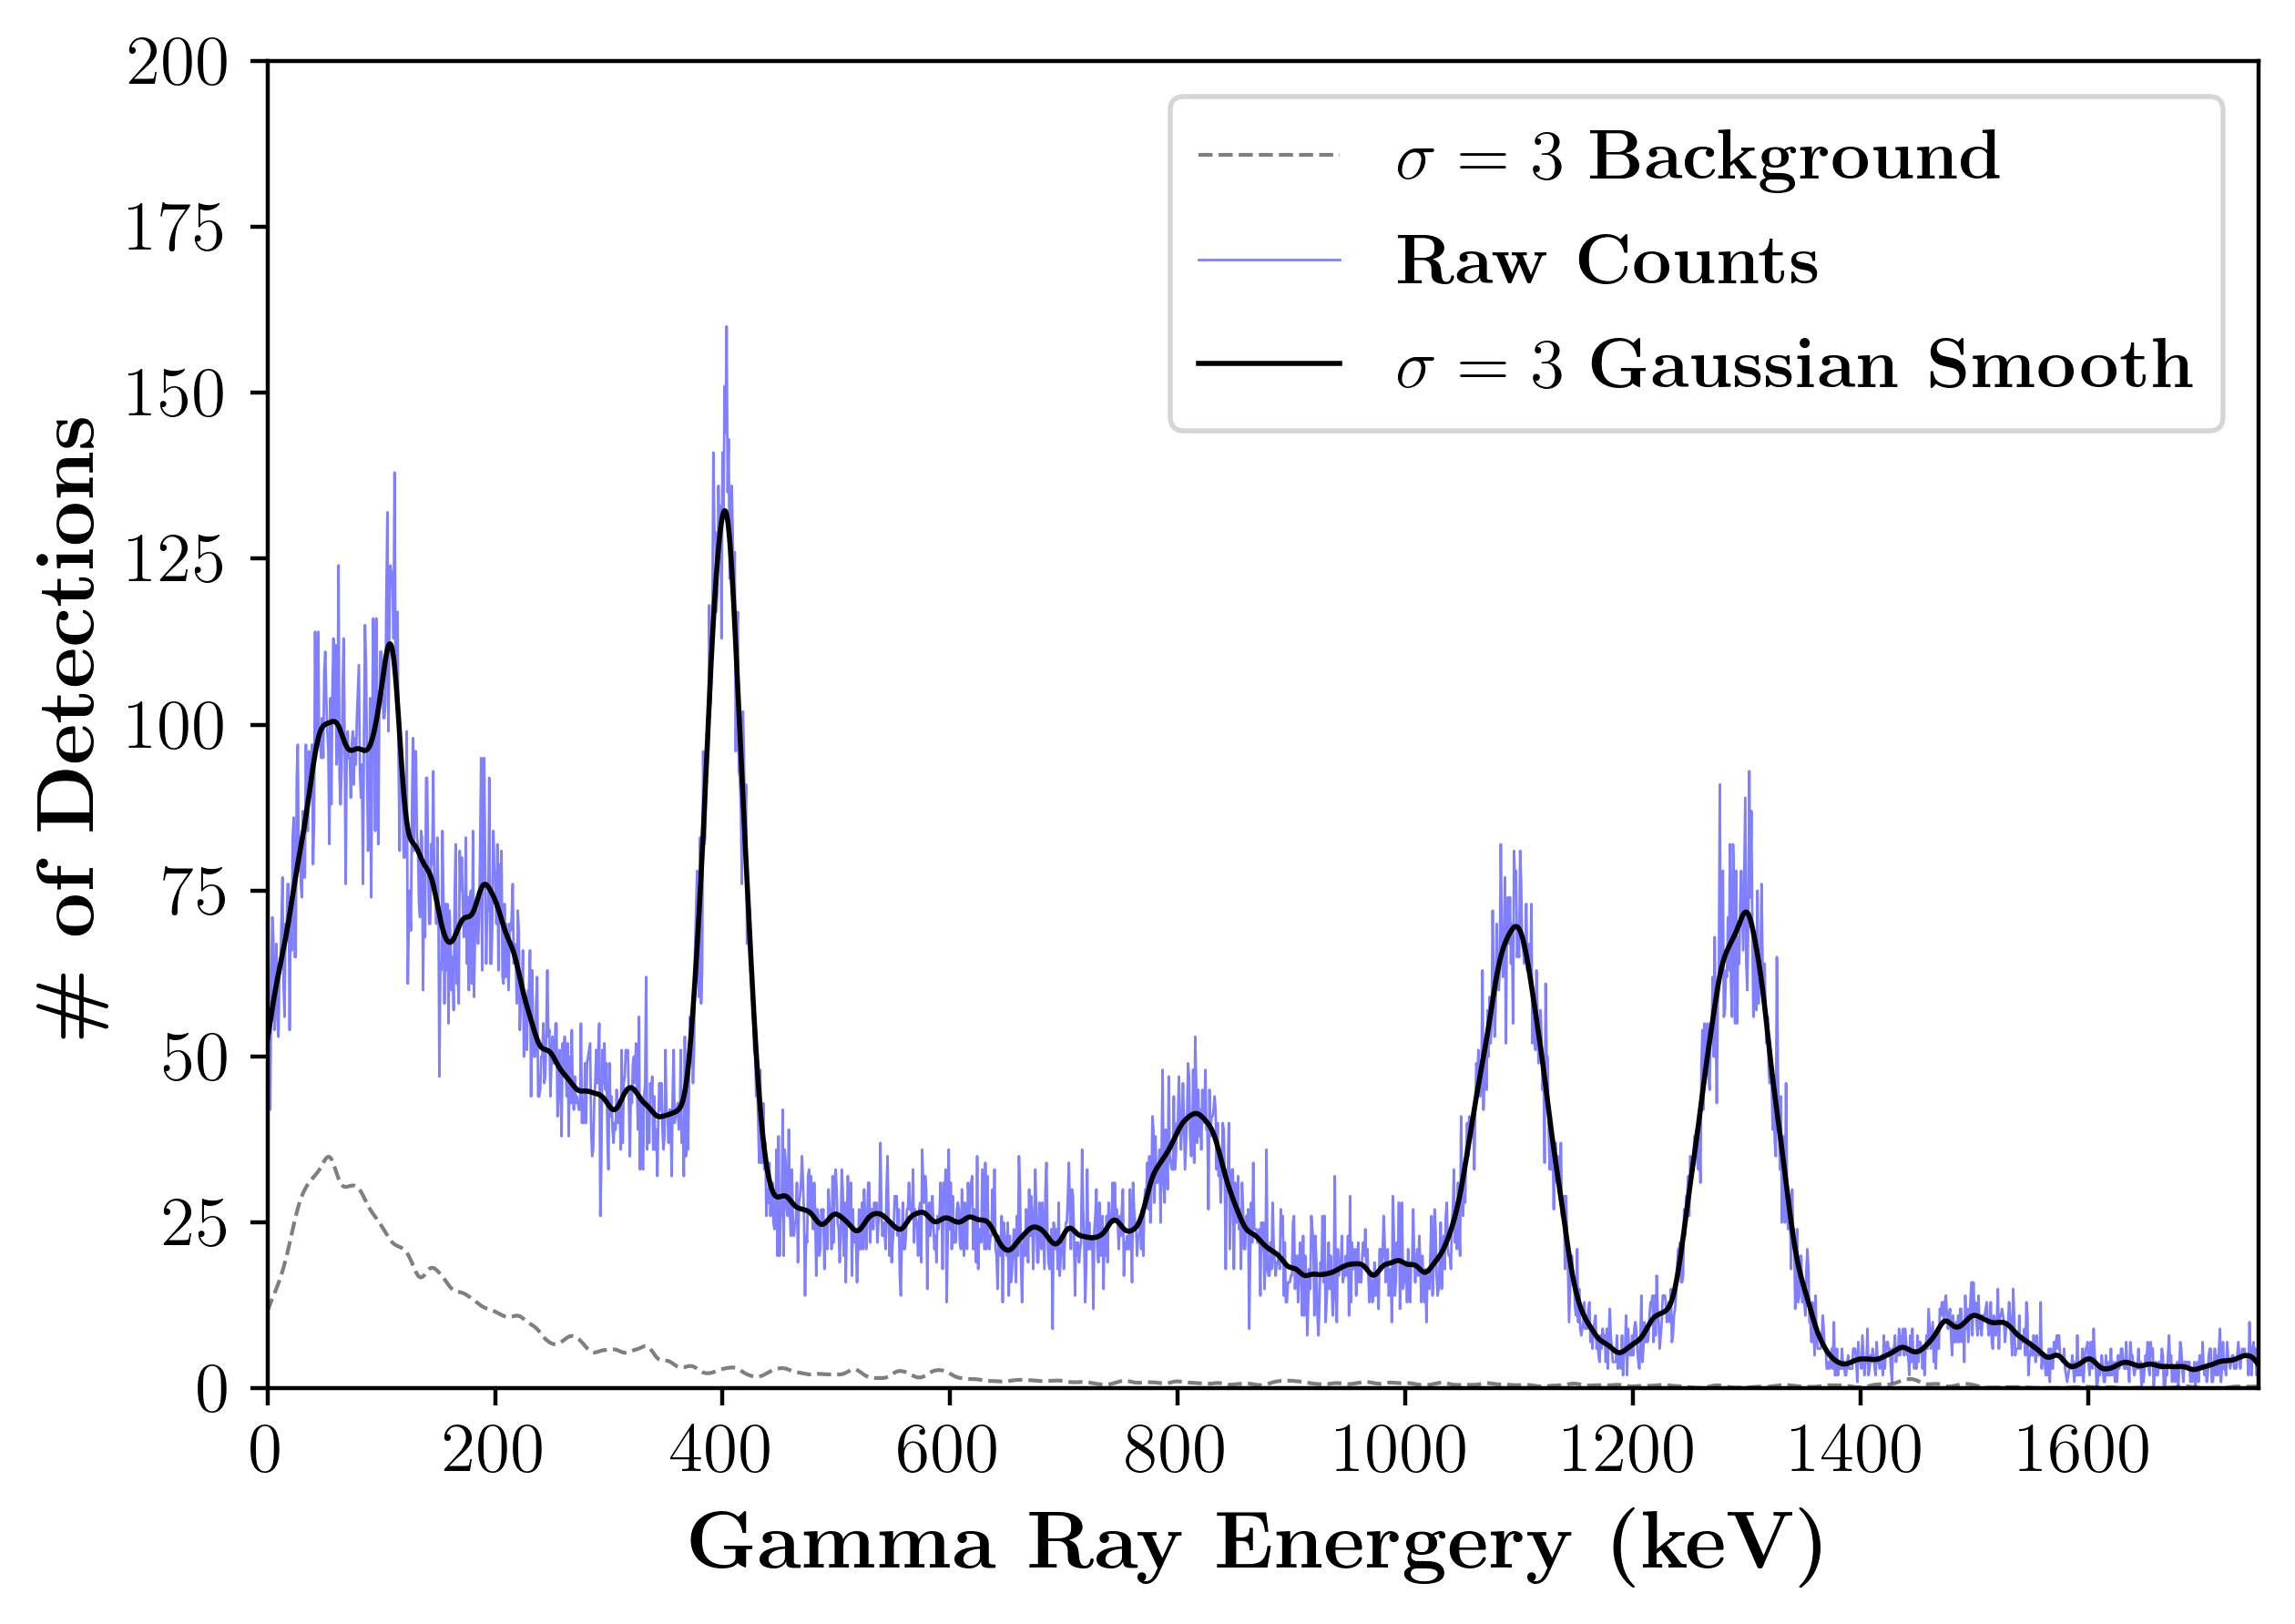
\includegraphics[width=0.49\textwidth]{figures/mystery_1_background_counts_overlay.png}}
        \hspace{\fill}
        \subfloat[Recording 2, hh:mm:ss, $T+$ minutes\label{subfig:mystery-recording-2}]{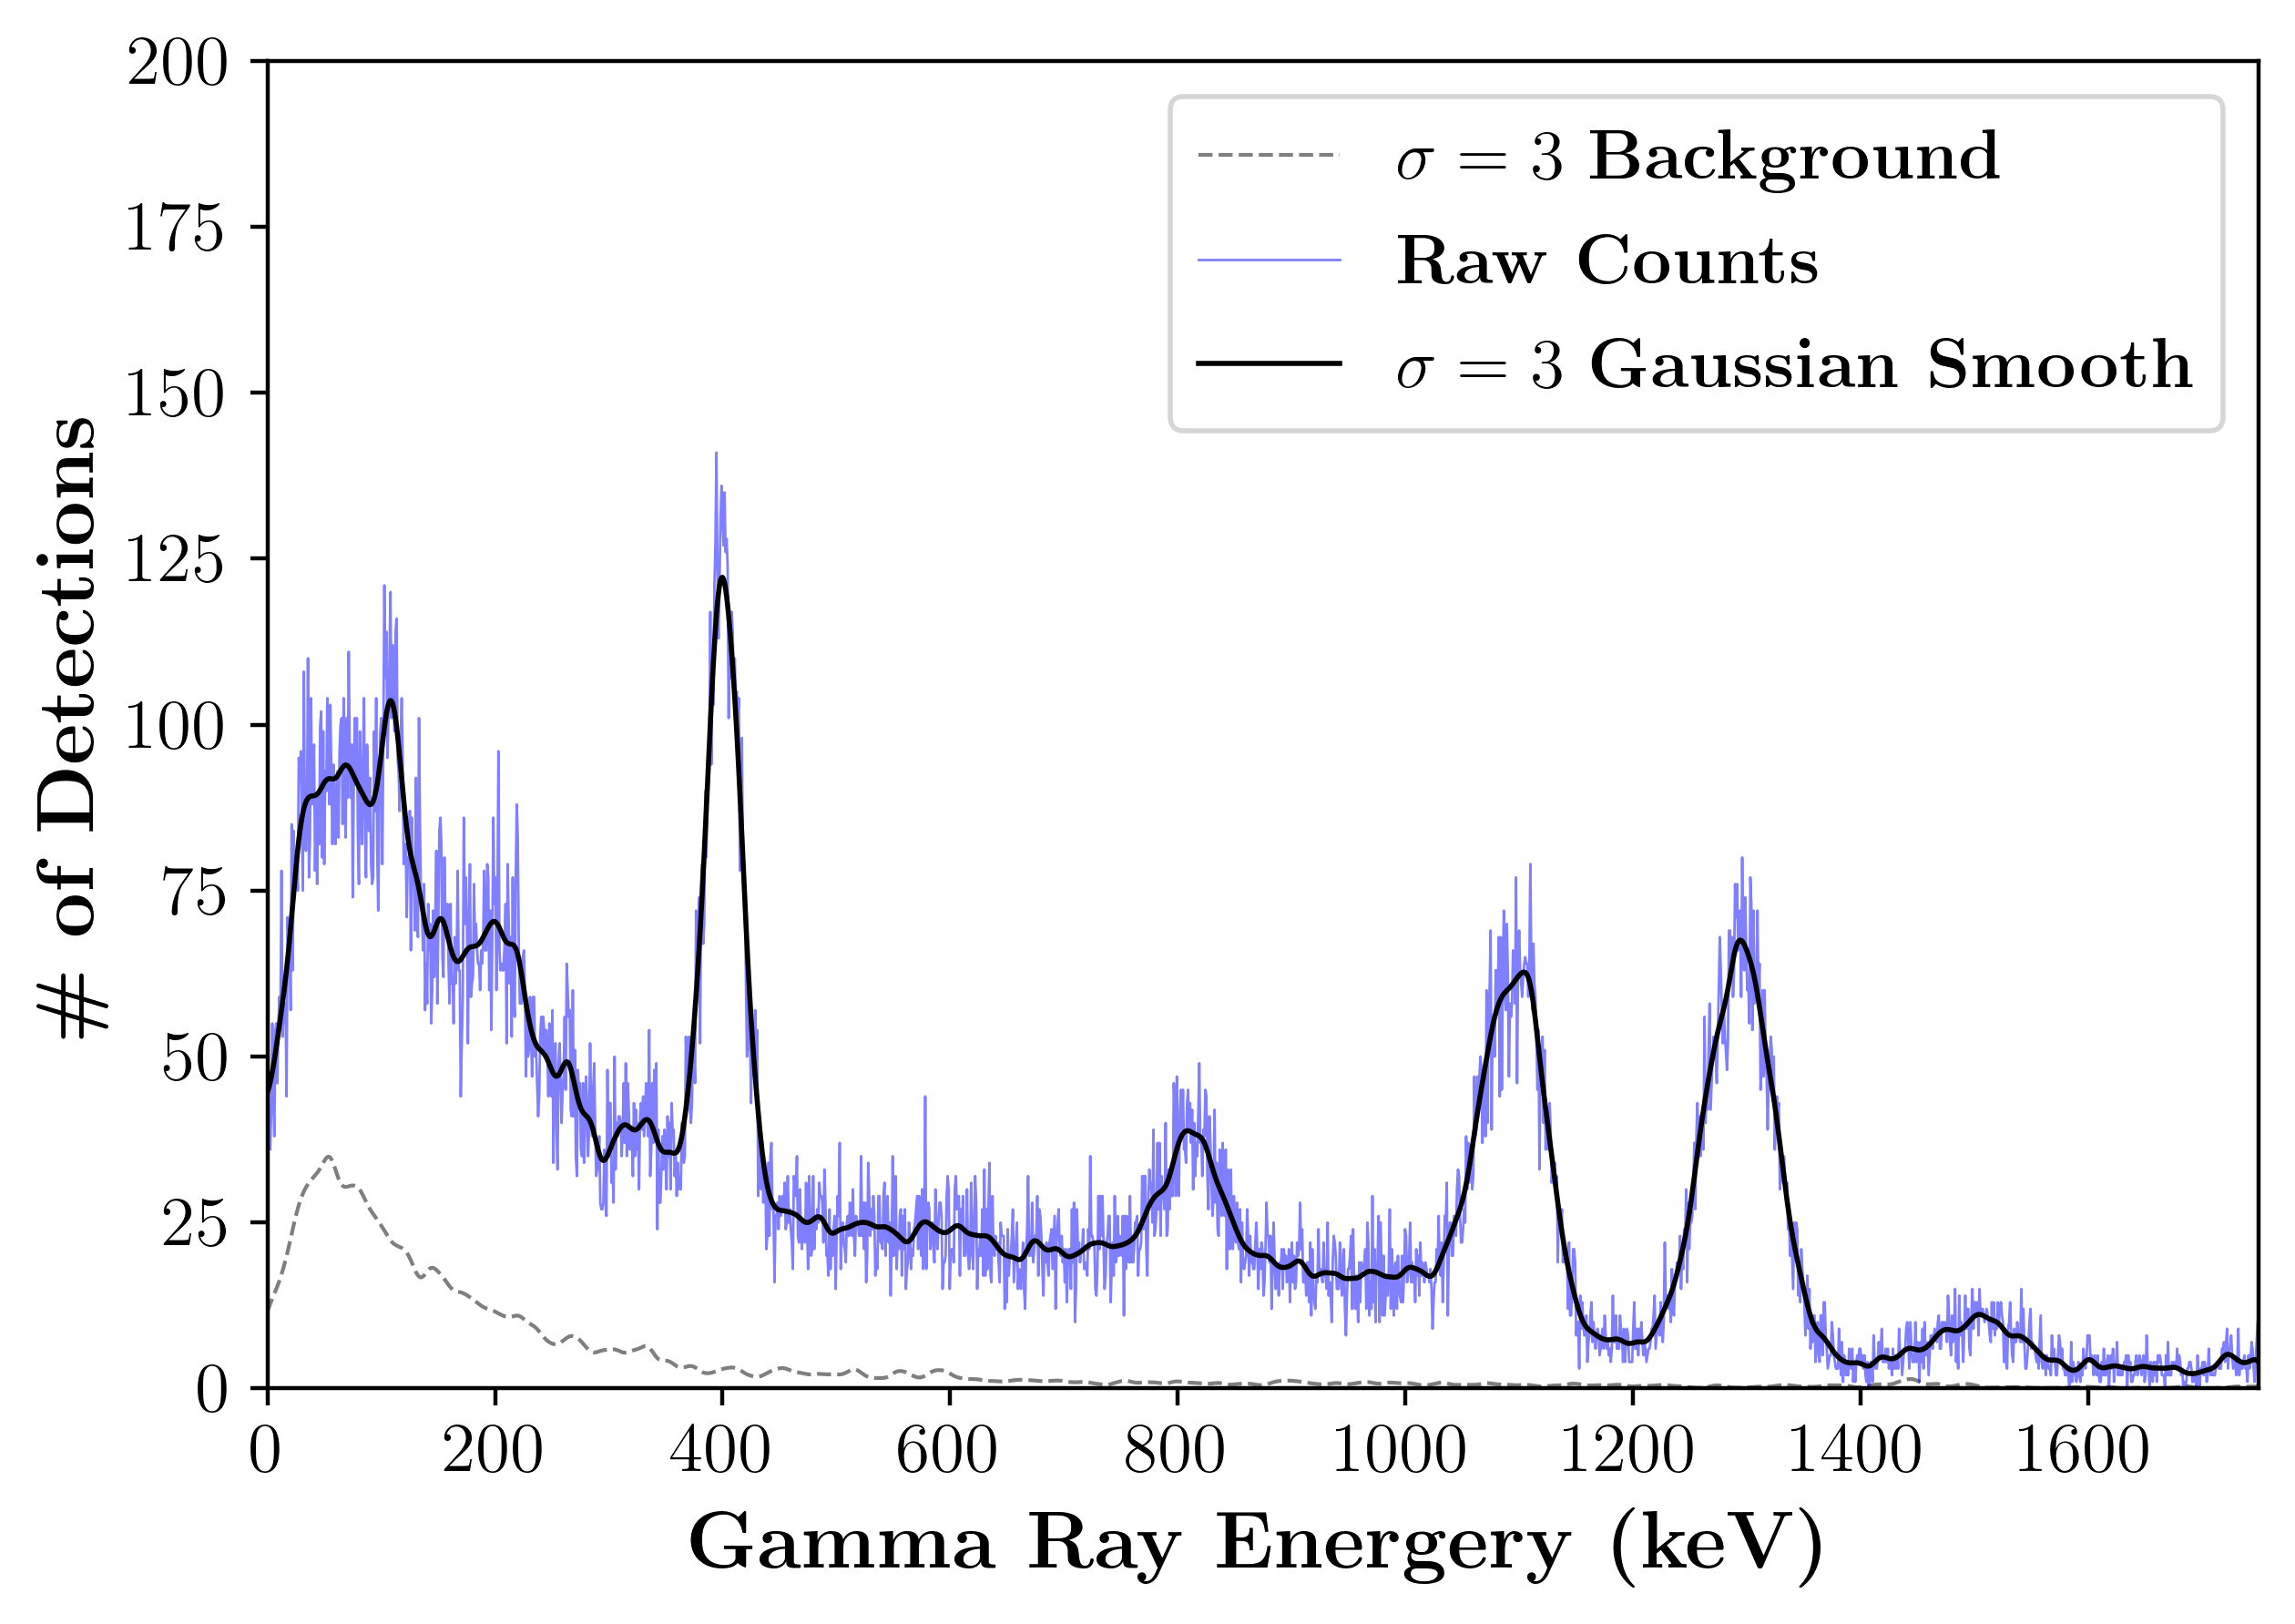
\includegraphics[width=0.49\textwidth]{figures/mystery_2_background_counts_overlay.png}}\\
        \subfloat[Recording 3, hh:mm:ss, $T+$ minutes\label{subfig:mystery-recording-3}]{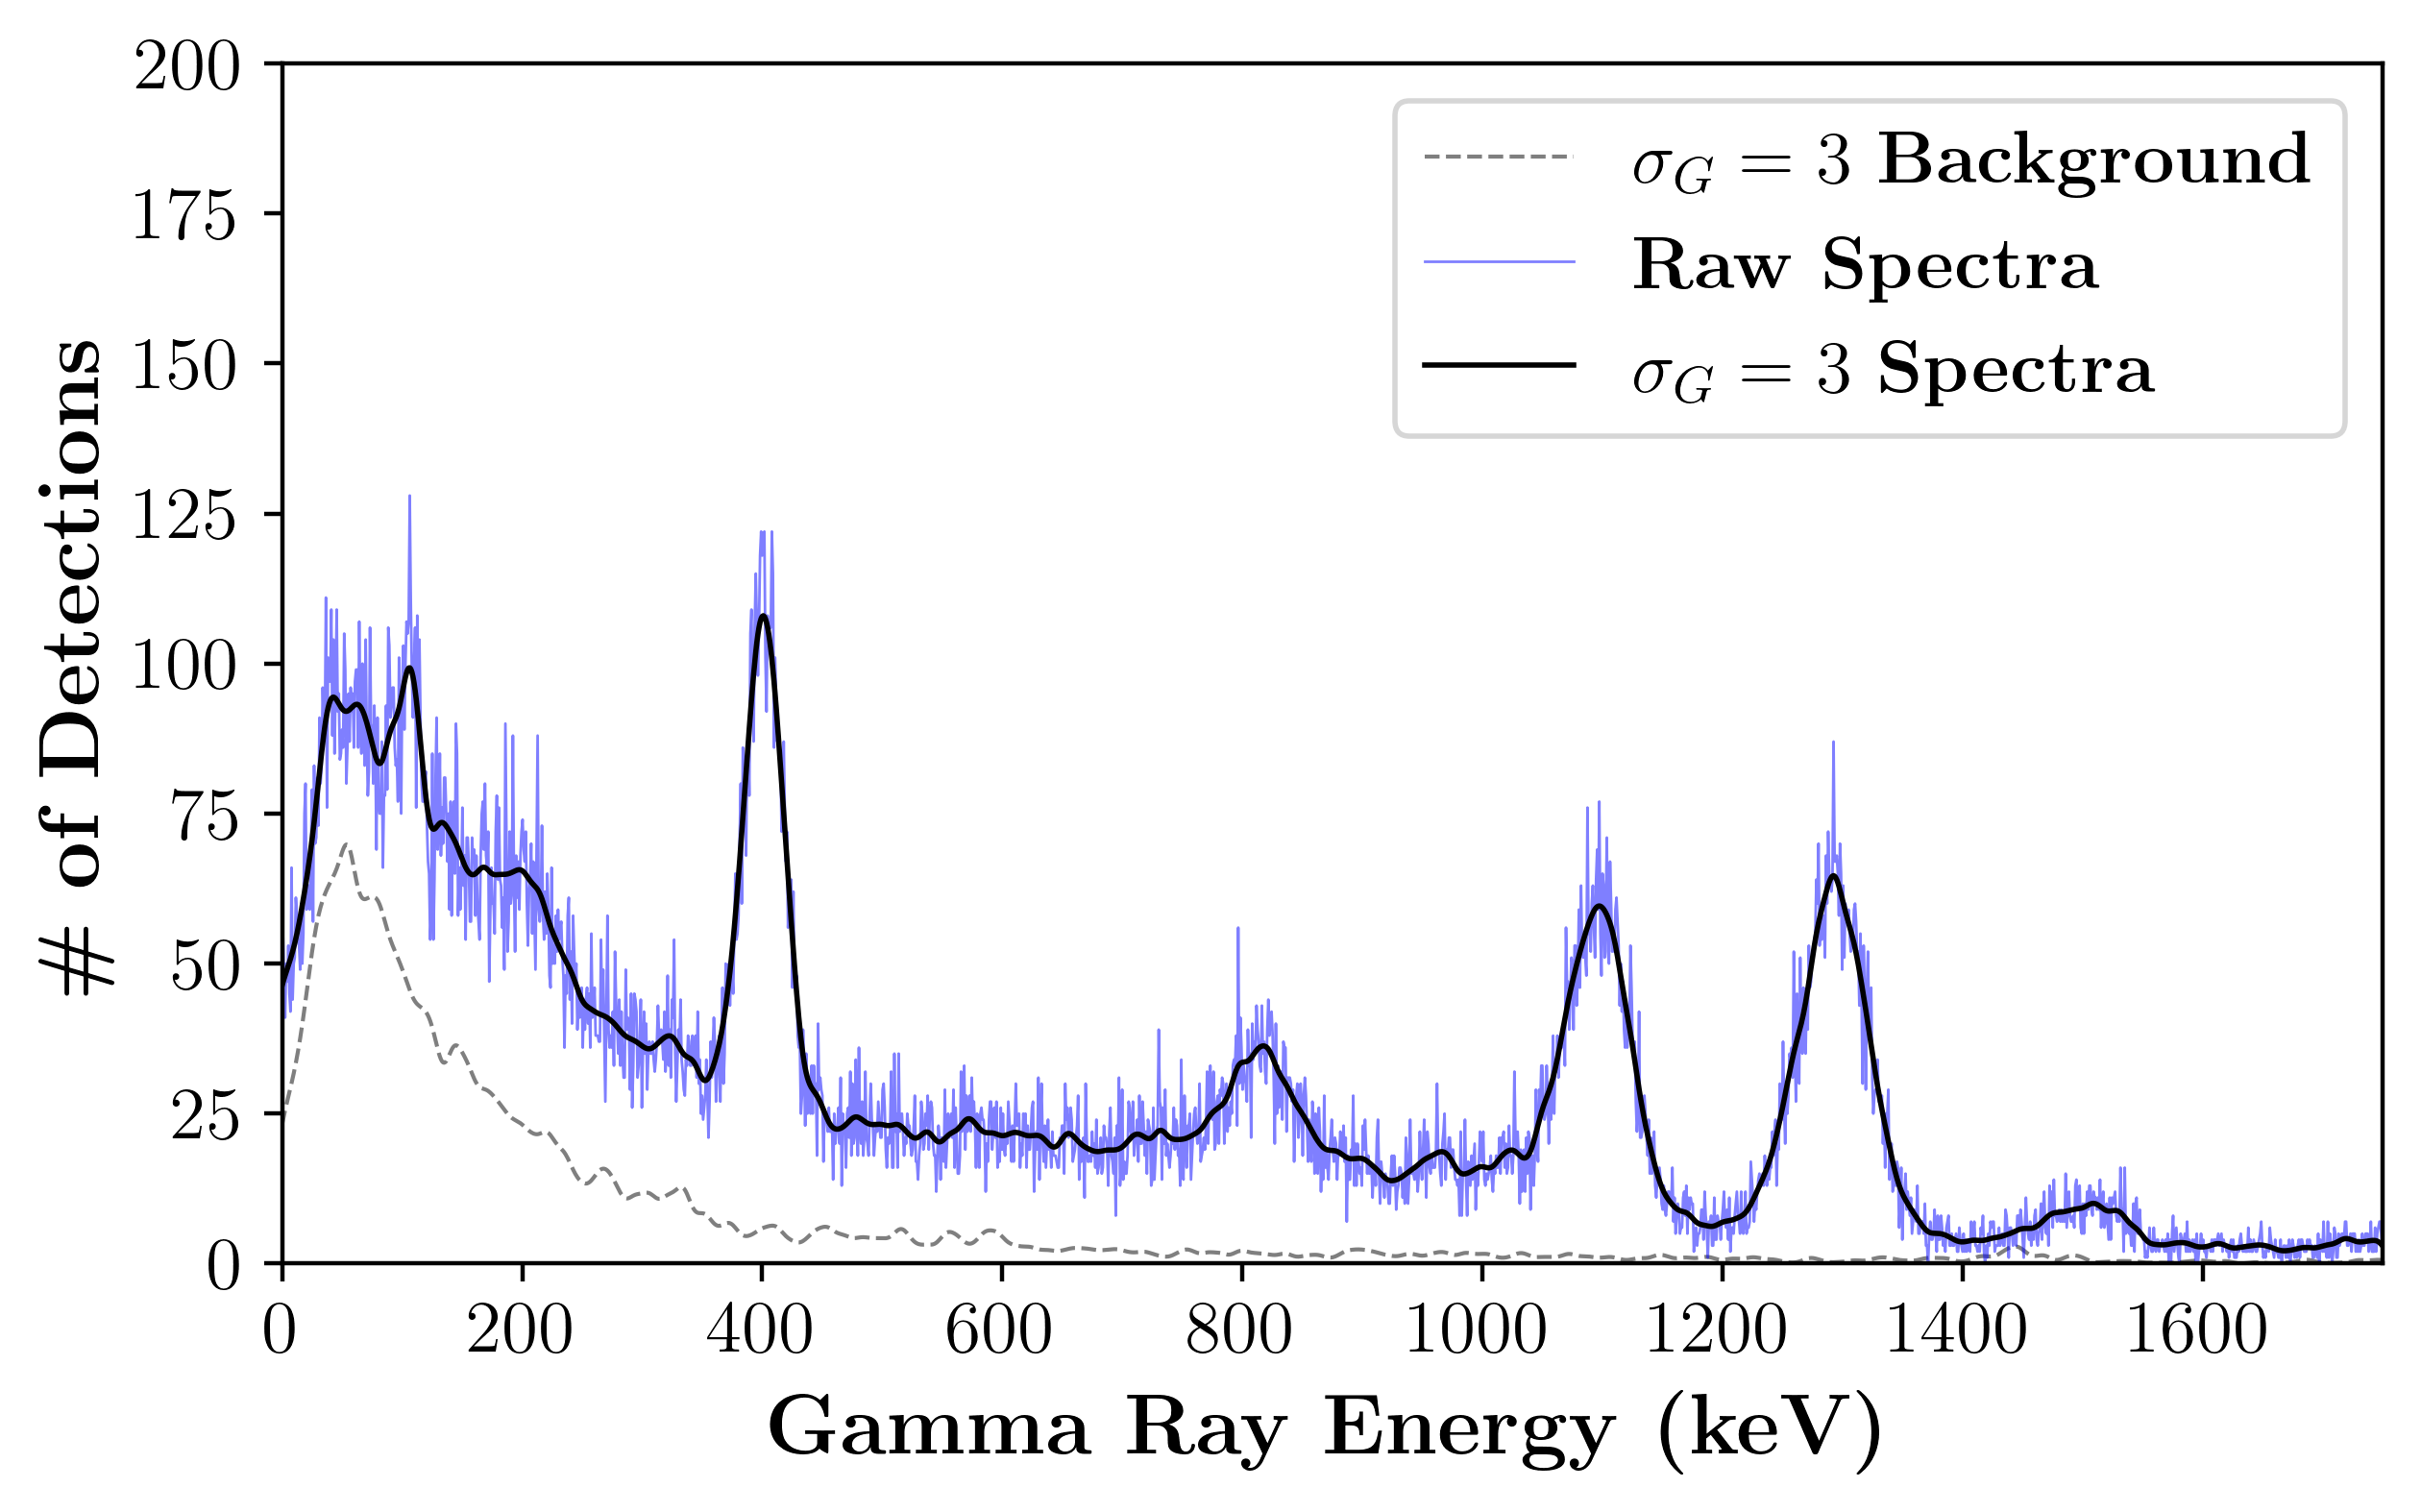
\includegraphics[width=0.49\textwidth]{figures/mystery_3_background_counts_overlay.png}}
        \hspace{\fill}
        \subfloat[Recording 4, hh:mm:ss, $T+$ minutes\label{subfig:mystery-recording-4}]{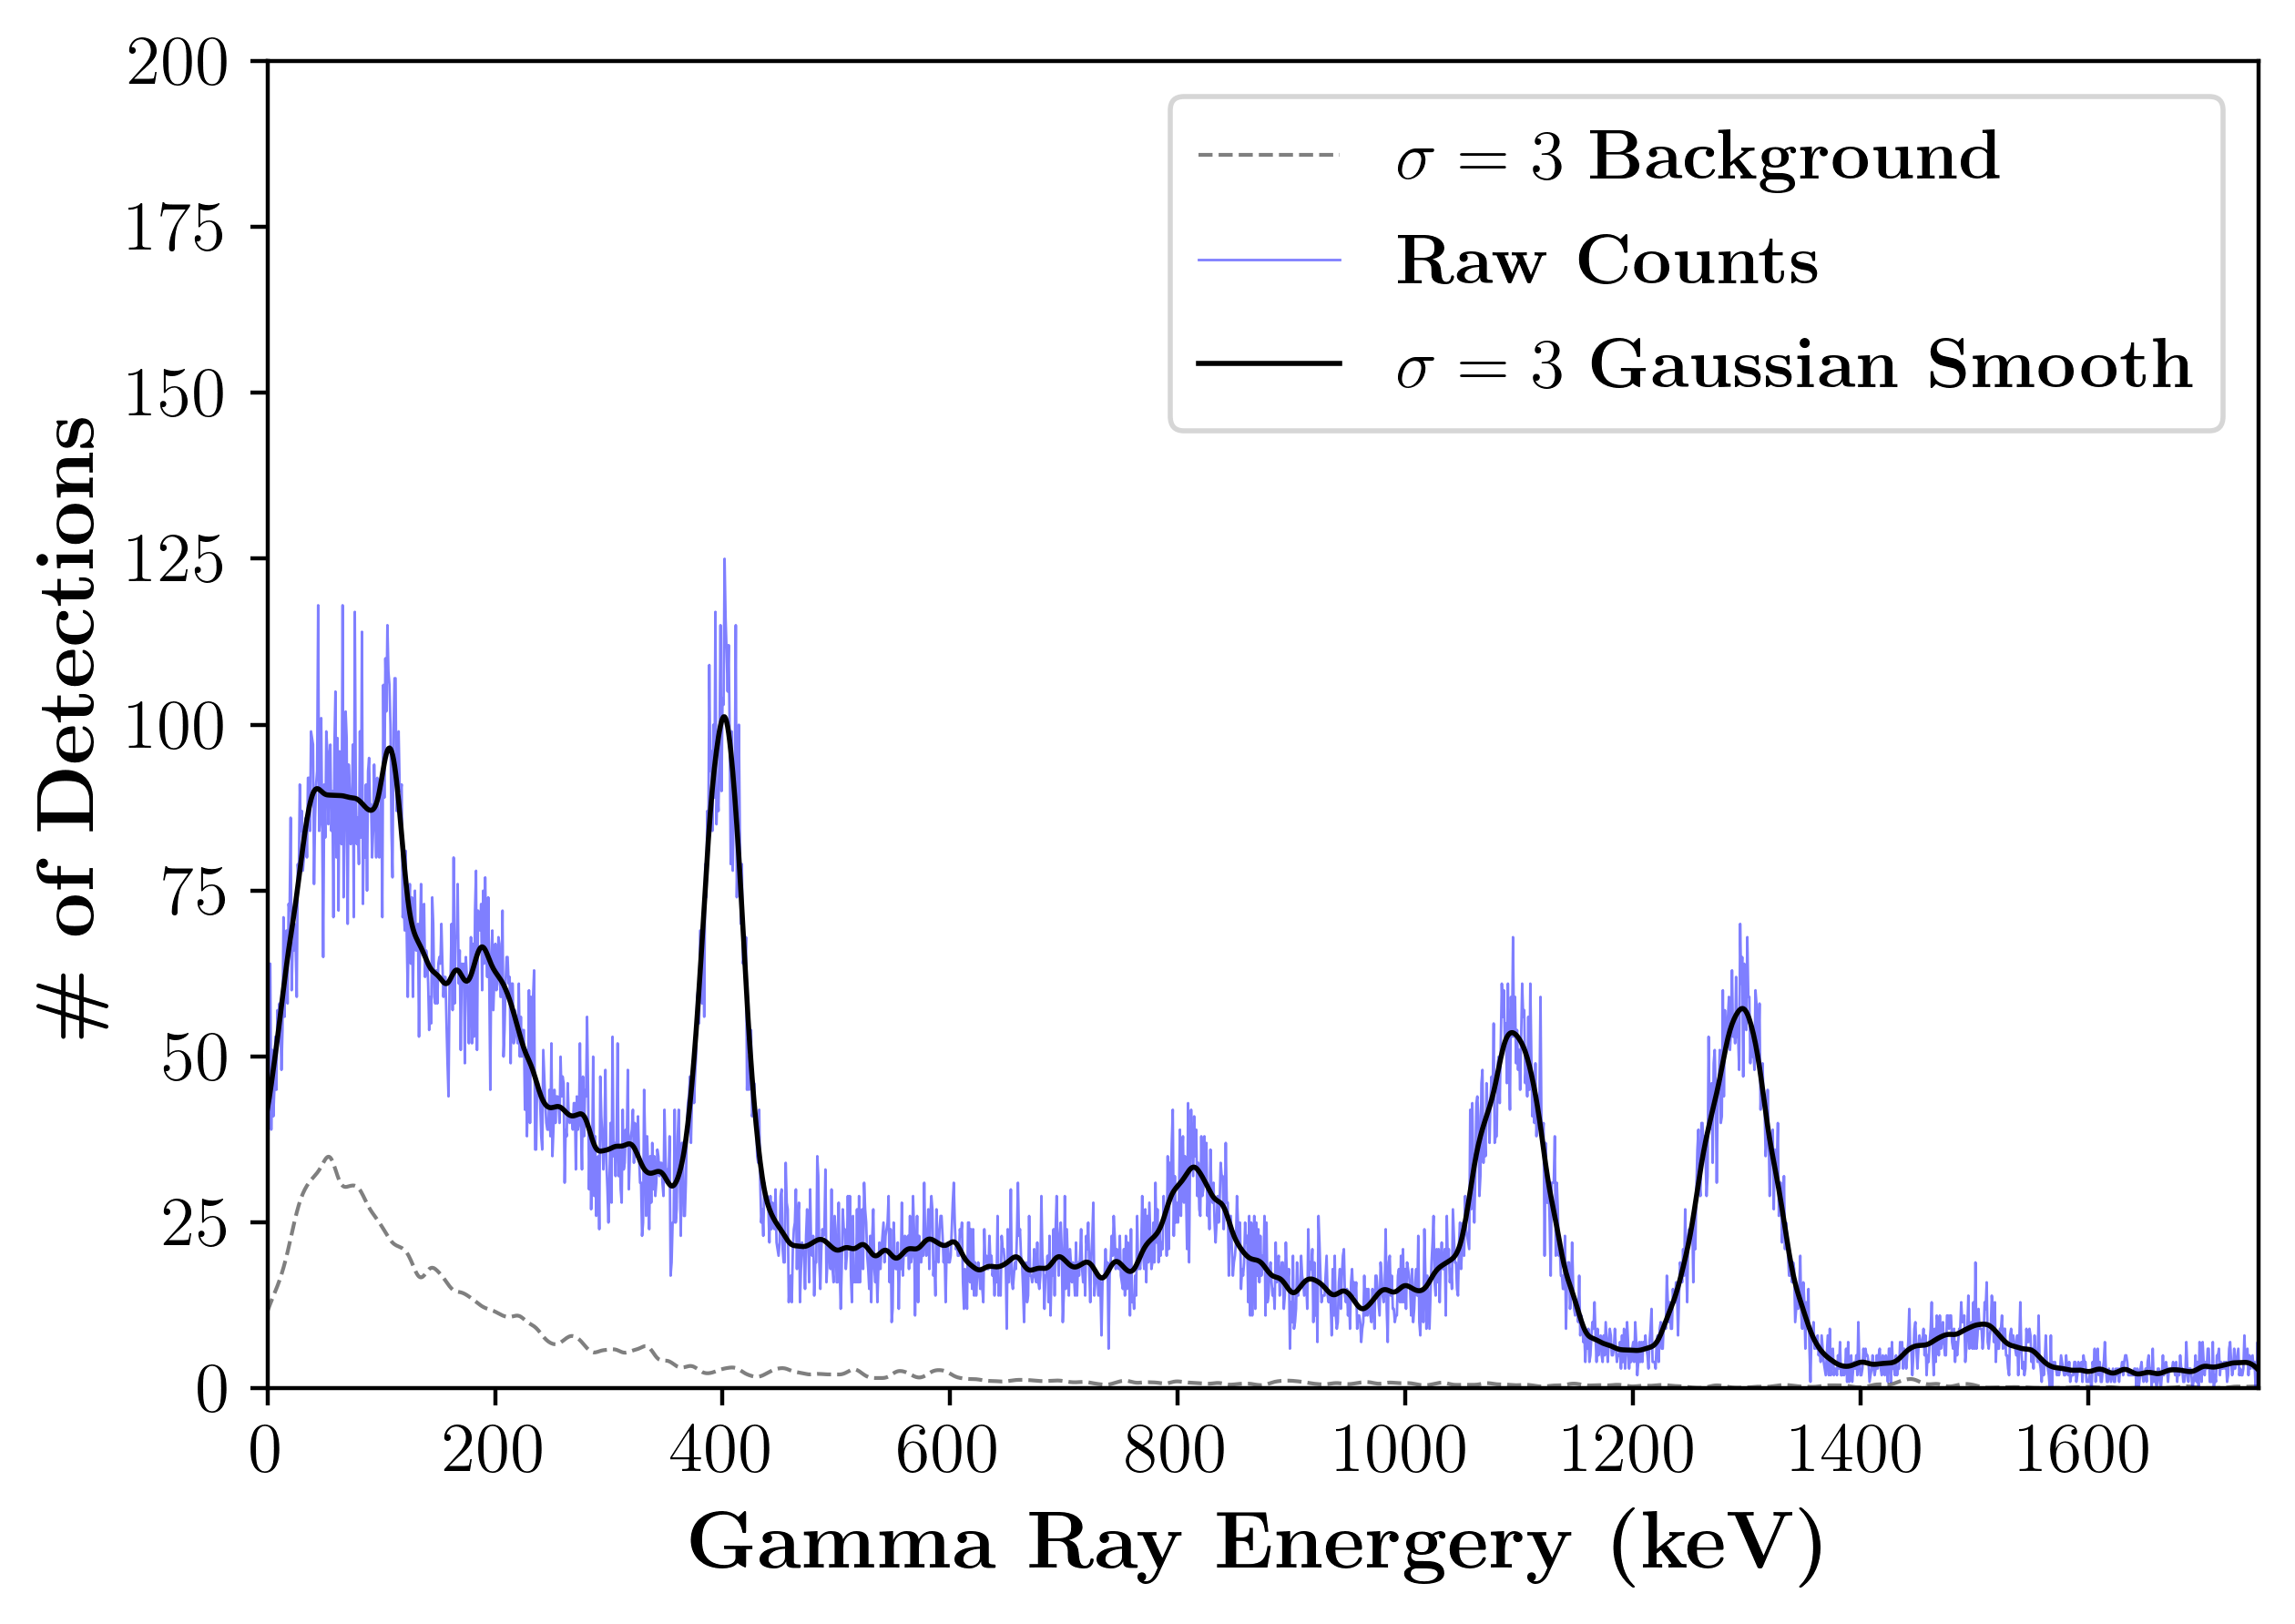
\includegraphics[width=0.49\textwidth]{figures/mystery_4_background_counts_overlay.png}}\\
        \subfloat[Recording 5, hh:mm:ss, $T+$ minutes\label{subfig:mystery-recording-5}]{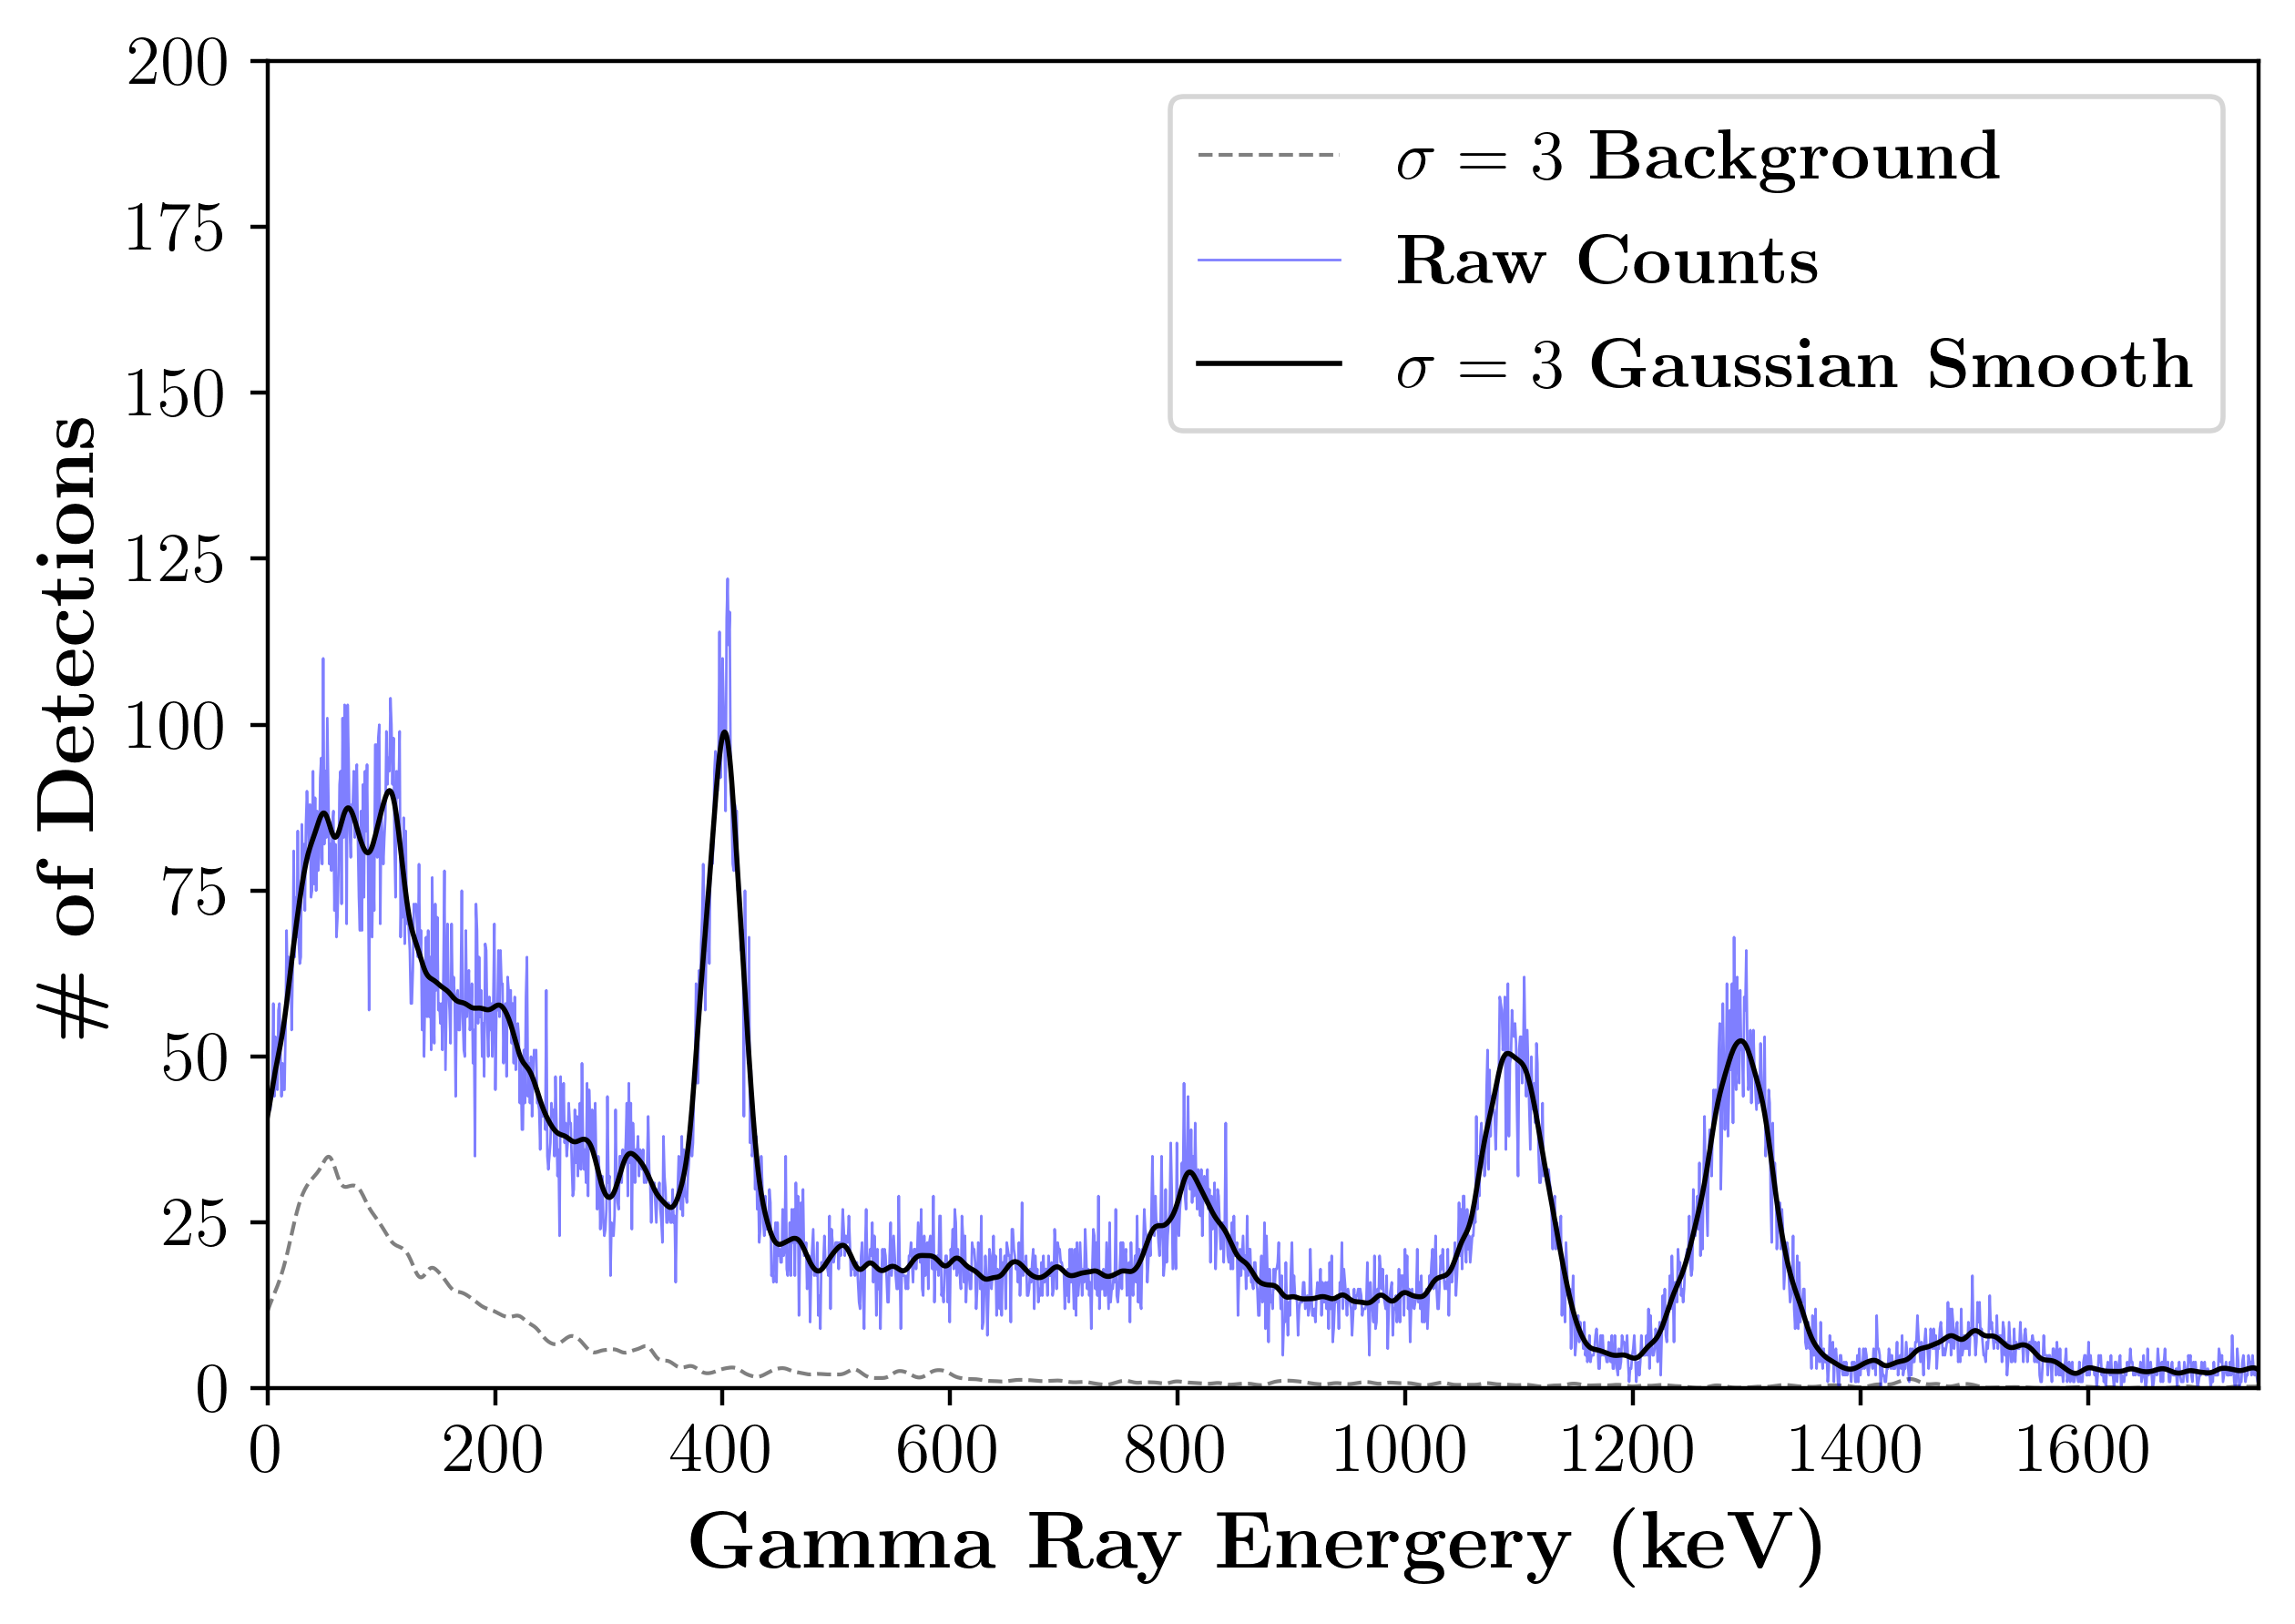
\includegraphics[width=0.49\textwidth]{figures/mystery_5_background_counts_overlay.png}}
        \hspace{\fill}
        \subfloat[Recording 6, hh:mm:ss, $T+$ minutes\label{subfig:mystery-recording-6}]{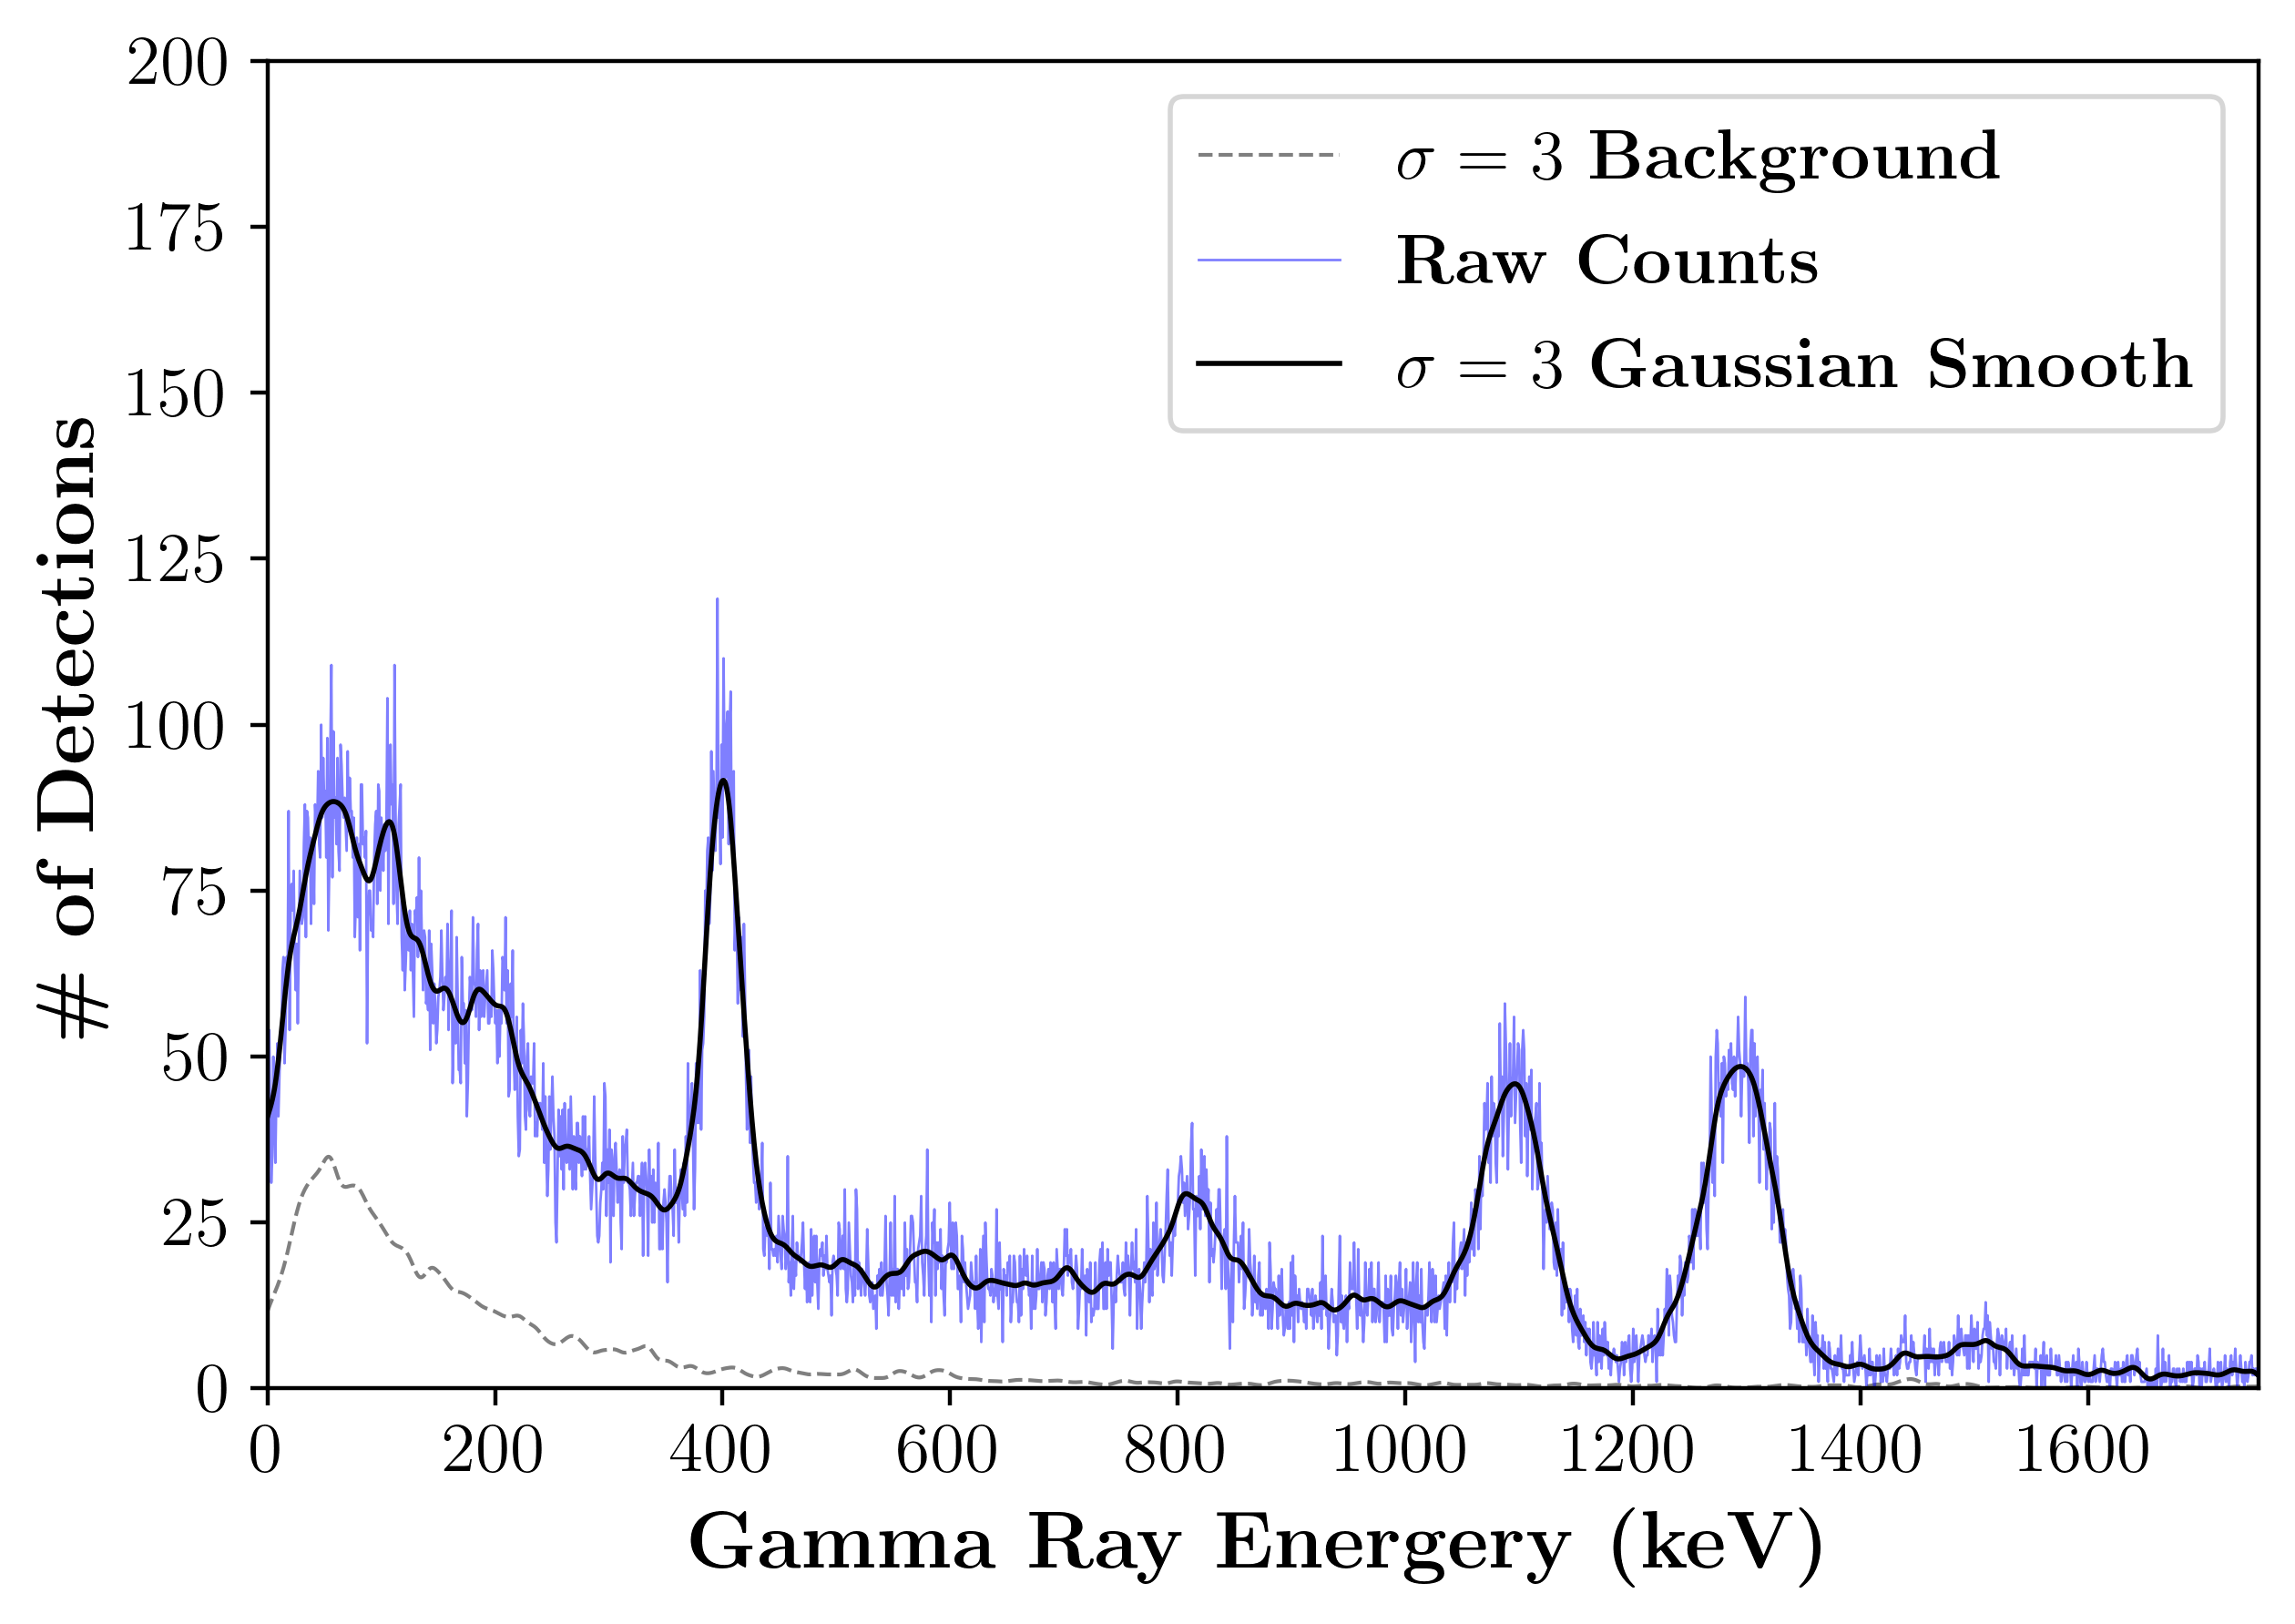
\includegraphics[width=0.49\textwidth]{figures/mystery_6_background_counts_overlay.png}}
        \caption{Raw count data for each recording of gamma rays from the unknown isotope.}
    \end{figure}
    ss
\end{document}